\section{Introduction}

ppcemu-system is a full system simulator of an MPC7447A/MPC107 (PowerPC) based board with Linux boot capability. The simulated board is very similar to a PowerMac G4 PCI machine. Computations on IEEE 754 floating point numbers are emulated using simfloat. Altivec instructions are currently decoded but not implemented. The running PowerPC application is a PowerMac Linux Kernel and all the applications installed on the hard disk image and/or the initial RAM disk image. Software running on the simulated hardware can be debugged by connecting a GDB client to the simulator through the GDB serial remote protocol. The GDB client can be either the standard text based client (i.e. command gdb), a graphical front-end to GDB (e.g. ddd), or even Eclipse CDT.

\begin{figure}[!h]
	\begin{center}
		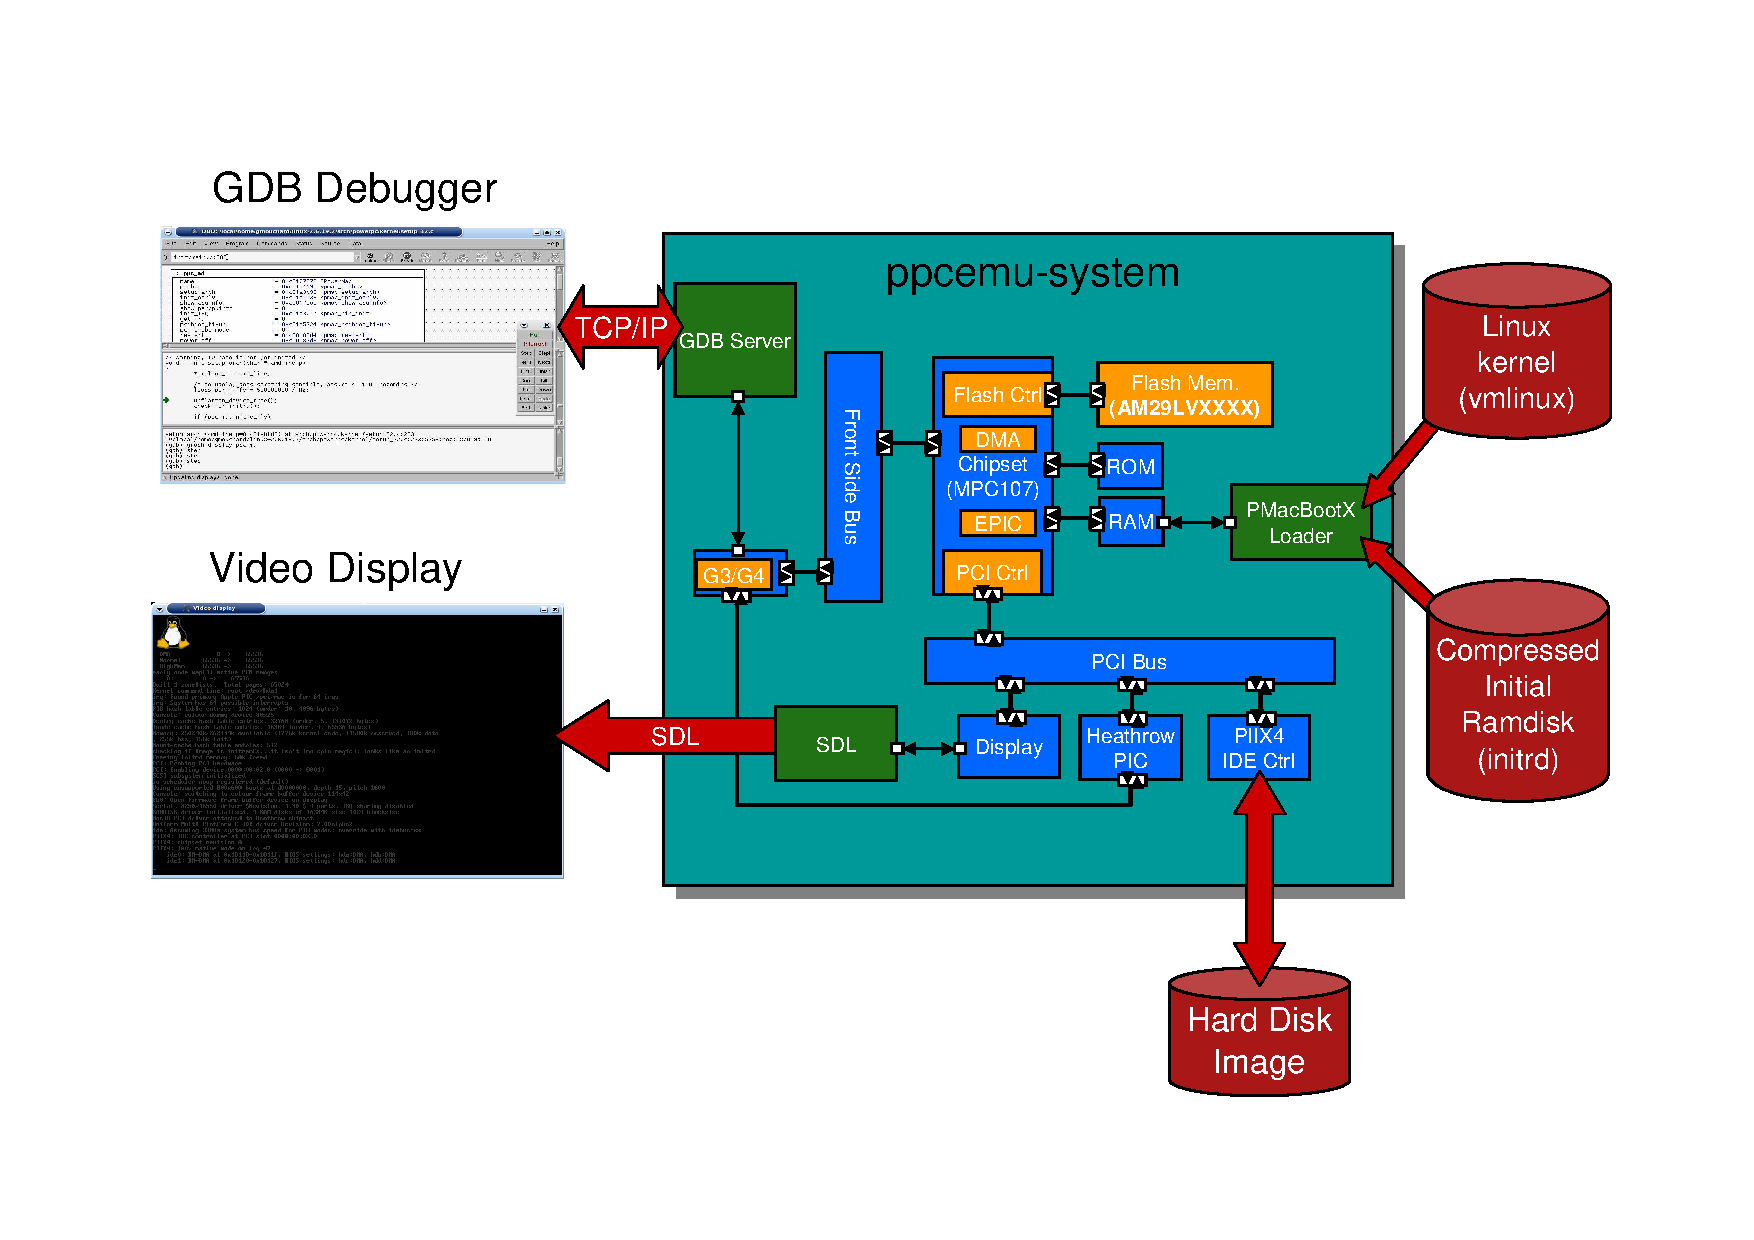
\includegraphics[width=\textwidth]{ppcemu_system/fig_ppcemu_system.pdf}
	\end{center}
	\caption{ppcemu-system simplified schematic.}
	\label{fig:ppcemu_system}
\end{figure}

\section{Simulated configuration}

The simulator is composed of the following modules:
\begin{itemize}\addtolength{\itemsep}{-0.40\baselineskip}
\item PowerPC CPU configured as an MPC7447A
\item snooping bus (front side bus)
\item MPC107 chipset
\item memory
\item rom
\item AM29LVxxx flash memory configured as an AM29LV800
\item PCI bus
\item PIIX4 IDE controller
\item Heathrow Programmable Interrupt Controller
\item Video frame buffer display
\item PCI-to-ISA bridge
\item i8042 keyboard controller
\end{itemize}

The simulator uses the following services:
\begin{itemize}\addtolength{\itemsep}{-0.40\baselineskip}
\item SDL
\item PowerMac Linux kernel loader
\item GDB Server
\item Inline debugger
\item SystemC Time
\item Host Time
\item Power Estimators (for ITLB, DTLB, IL1, DL1 and L2)
\end{itemize}

\section{Using the simulator}

Usage: \texttt{ppcemu-system [<options>] <linux kernel> [linux kernel arguments]}

‘linux kernel’ is an ELF32 uncompressed Linux kernel (vmlinux) A ‘Mac OS BootX’ loader is emulated instead of directly running an open firmware and a boot loader

Options:

\begin{itemize}

\item Starting the inline debugger

\texttt{--inline-debugger}
\texttt{-d}

\item Starting a GDB server

\texttt{--gdb-server <TCP port>}
\texttt{-g <TCP port>}

The GDB server will wait for a GDB client connection on the specified TCP port.

\item Defining the width (in pixels) of the video display

\texttt{--screen-width <width>}
\texttt{-x <width>}

\item Defining the height (in pixels) of the video display

\texttt{--screen-height <height>}
\texttt{-y <height>}

\item Capturing the video display as Windows bitmap (.BMP) files

\texttt{--capture <bitmap out filename>}
\texttt{-u <bitmap out filename>}

\item Defining the architecture description to be used by the GDB server

\texttt{--gdb-server-arch-file <arch file>}
\texttt{-a  <arch file>}

\item Defining the device tree to be used by the PowerMac Linux kernel loader

\texttt{--device-tree}
\texttt{-t  <devtree file>}

\item Defining the video display refresh period (in milliseconds)

\texttt{--video-refresh-period <period>}
\texttt{-f <period>}

\item Disabling the video display

\texttt{--no-video}
\texttt{-n}

\item Defining the number of instructions to simulate before exiting

\texttt{-i <count>}
\texttt{--max:inst <count>}

\item Enabling power estimation for ITLB, DTLB, IL1, DL1, and L2

\texttt{-p}
\texttt{--power}

\item Defining the compressed initial ramdisk image to be loaded by the PowerMac Linux kernel loader

\texttt{-r <file>}
\texttt{--ramdisk <file>}

\item Defining the IDE disk image (ide0)

\texttt{-c <file>}
\texttt{--disk:image0 <file,file,...>}

\item Redirecting the logger output into a file

\texttt{-l <file>}
\texttt{--logger:file <file>}

\item Enabling compression (gzip format) of the logger output

\texttt{-z}
\texttt{--logger:zip}

\item Redirecting the logger output to the standard error output

\texttt{-e}
\texttt{--logger:error}

\item Redirecting the logger output to the standard output

\texttt{-o}
\texttt{--logger:out}

\item Displaying the integrated help

\texttt{--help}
\texttt{-h}

\end{itemize}